\section{Market Design for a Self-Incentivizing Network}
\label{sec:designs}

\begin{itemize}

\item Desired properties

\begin{itemize}

\item Let anybody contribute capacity

\item Allow users with different utility functions to interact (flow completion time vs.~jitter)

\item Allow users to buy guarantees (and not get swindled)

\end{itemize}

\item Simulation experiments to test whether the one-layer market has each desired property?

\item Measure outcome quality (vs.~SRTF or other optimal), \# of roundtrips

\item Sketch of multi-layer design

\end{itemize}

\begin{figure}
%\vspace{\baselineskip}
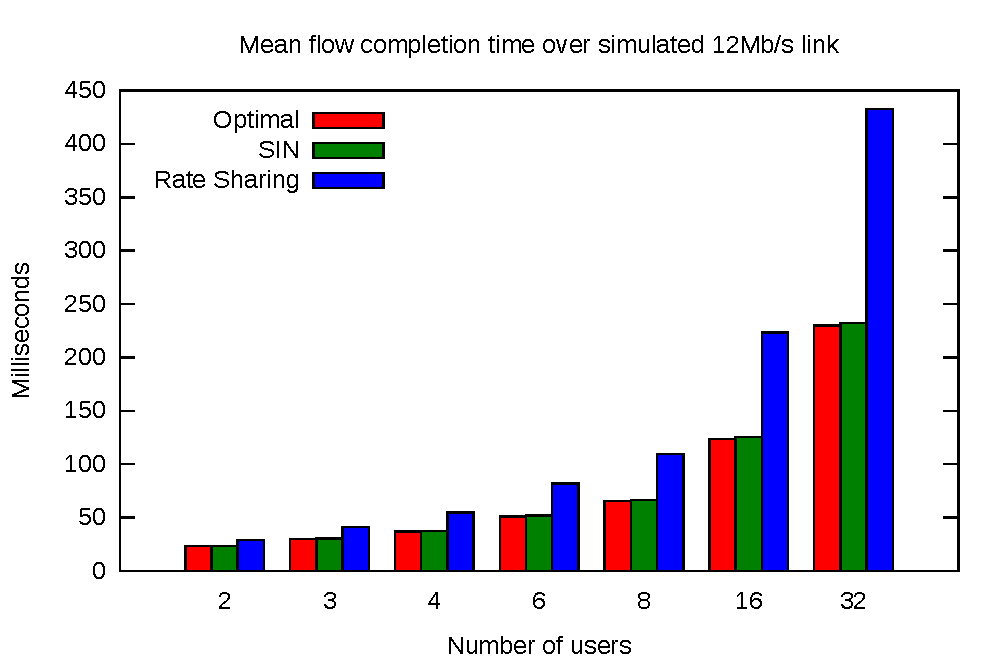
\includegraphics[width=\columnwidth]{plots/delay_over_srtf.pdf}
\caption{The blue line represents the efficient frontier, which here is defined entirely by the RemyCCs.}
\label{f:delay_over_srtf}
\end{figure}

\begin{figure}
%\vspace{\baselineskip}
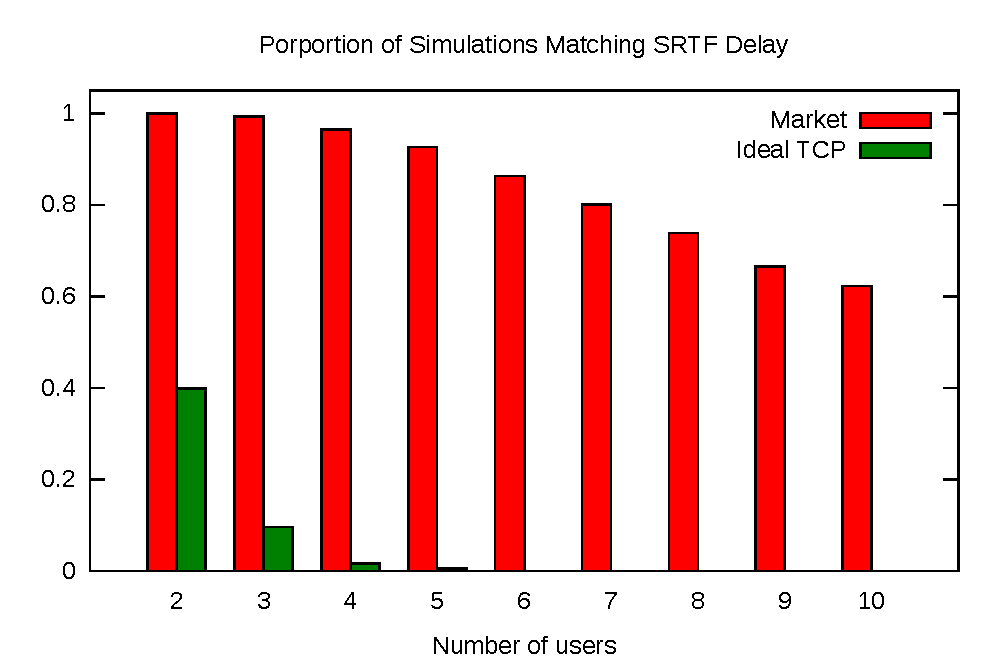
\includegraphics[width=\columnwidth]{plots/percent_match_srtf.pdf}
\caption{The blue line represents the efficient frontier, which here is defined entirely by the RemyCCs.}
\label{f:percent_match_srtf}
\end{figure}

Testing.
